\documentclass[a4paper]{report}

\usepackage{graphicx}
\usepackage[english]{babel}
\usepackage[utf8]{inputenc}
\usepackage[T1]{fontenc}
\usepackage{ragged2e}
\usepackage{hyphenat}
\usepackage{lmodern}
\usepackage{fancyhdr}
\usepackage[toc,page]{appendix}
\usepackage{tabularx}
\usepackage{float}
\usepackage{gensymb}

\begin{document}
    \centering
    \LARGE{\textsc{VIETNAM AVIATION ACADEMY}} \\
    \vspace{3mm}
    \normalsize{Department of Telecomunication - Electronics Engineering Technology} \\
    \vspace{3mm}
    \large{LOCATION IN HO CHI MINH CITY} \\
    \vspace{3mm}
    
\includegraphics[scale=0.3]{logo.jpg} \\
    \vspace{3mm}
    \normalsize{PROJECT REPORT:} \\
    \vspace{15mm}
    \huge{\textbf{"Circuit Remote Controlled Using Infarred Light"}} \\
    \vspace{20mm}
    \normalsize{Written by} \\
    \vspace{3mm}
    \large{\textit{Nguyen Van Anh Tuan}} \\ 
    \vspace{3mm}
    \textit{\large{Roll.No.1753020018}} \\
    \vspace{15mm}
    \textbf{\large{Under the guidance of}} \\
    \vspace{10mm}
    \centerline{\textbf{\large{Master Cao Xuan Kim Anh}}}

    % Lines down here to set footer and header. 
    \pagestyle{fancy}
    \fancyhf{}
    \rhead{Report Project 1}
    \lhead{CaptainJAV}
    \cfoot{\today}
    \renewcommand{\headrulewidth}{2pt}
    \renewcommand{\footrulewidth}{1pt}

    \newpage
    \centerline{\textbf{\huge{PREAMBLE}}} 
    \vspace{10mm}
    \begin{flushleft}
        In this day of advancement, we are indispensable remote control to control
        the devices we use every day as televisions, machines air conditioners, fan, etc.
        So how do remote controls work? Can control other objects in the distance? 
        Few know that the first remote control available during World War II. 
        Initially, people use RF technology (Radio Frequency) and then catch to start applying 
        IR (Infarred Remote) technology to the remote control. In today's life, we use 
        both types, however control remote use infarred in more often used. Let's see the principle operation 
        and construction of this remote control.
    \end{flushleft}
    \begin{flushright}
        \textbf{Auth. Nguyen Van Anh Tuan}
    \end{flushright}
    \thispagestyle{plain} % This command make this page have no header or footer.

    \newpage
    \tableofcontents

    \chapter{Introduction}
    \thispagestyle{fancy}
    \fancyhf{}
    \fancyhead[L]{CaptainJAV}
    \fancyhead[R]{Remote Controlled Using Infarred}
    \raggedright % Set all text to the left side.
    \rfoot{Page \thepage}
    \section{Preliminary introduce:} 
        With the current trend of modernization and industrialization, many modern technology 
        devices appear to help save time. We can mention as public technology of things 
        connected through the internet (Internet of Things) etc. But with expensive fees 
        are not suitable for the average consumer. From there, i founded simple solutions 
        with the same purpose and low cost.
        \linebreak
        \par In parallel, to supplement, to supplement the knowledge not studied 
        in school. From there, i selected "Remote Controlled Using Infarred" for the topic.
    \section{Objectives of the study:}
        To help reduce costs and supplement knowledge not researched at school.
    \section{Research Methods:}
        Find information on internet. \\
        Test on software. \\
        Construction circuit.


    \chapter{Find out theoretical related to the research}
    \thispagestyle{fancy}
    \fancyhf{}
    \fancyhead[L]{CaptainJAV}
    \fancyhead[R]{Remote Controlled Using Infarred}
    \rfoot{Page \thepage}
    \section{Application of remote controlled using infarred}
        Remote controlled now is using broadly, it use to controlled all wireless device. 
        Remotes and televisions are the best example for application of this recieve and transmitter 
        circuit. Or more application of this circuit. Beside that, we can see that remote controlled 
        can use with air conditioners, fans, or even use to turn on the lights in house...etc.
    \section{Define of Infarred (IR LED)}
        Infarred light (infarred ray) is the light we can't see it by our eyes, 
        they have wavelength from 700nm to 1mm. The infarred light have transmittion speed 
        is equal to lightspeed.
        \linebreak
        \par The infarred can transmit many signal channels. It is widely 
        applied in industry.
        \linebreak
        \par The amount of information that it can gain is 3 megabit/s. The 
        amount of information transmit with infarred light is many times larger 
        compared to the electromagnetic waves people still use.
        \linebreak
        \par Infarred rays are easily absorbed, poor penetration. In the word control 
        far by infarred, the beam emits a narrow, directed direction, so when recieve 
        must be in the right direction to use it.
        \linebreak
        \par Infarred wave have characteristics such as light (focusing through the lens, focal distance...). 
        Normal light and infarred light differ very clearly in light through the material.
        \linebreak
        \par Other than emitting invisible infarred light, IR Led look like a normal led and also
        works like a normal Led, it means it will consume 20mA and 3 Volts.
        \linebreak
        \par Besides that infarred is divided by wavelength into three main regions. However, follow the US classification is divided into 5 areas as follow: \\ 
        \vspace{3mm} 
        \begin{table}[ht]
            \centering
            \begin{tabular} { | p{1cm} | l | p{2cm} | p{2cm} | p{2cm} | p{3cm} | }
            \hline
            Name &Acronym &Wavelength &Frequency &Photon Energy &Featured \\ 
            \hline
            Near Infarred &NIR &750nm to 1.4$\mu$m &214-400THz &886-1653 meV &Determined by the absorption of water.Used in fiber optic telecomunications. \\ 
            \hline
            Short waves infarred &SWIR &1.4-3$\mu$m &100-214THz &413-886meV &Absorbed domestic increase significantly as of 1.45$\mu$m. Range 1.53-1.56$\mu$m is spectral region currently in use much in the far informed long road. \\ 
            \hline
            Medium waves infarred &MWIR &3-8$\mu$m &37-100THz &155-413meV &This band is called is thermal infarred, but it only detects slightly higher temperatures than body temperatures. \\ 
            \hline
            Long waves infarred &LWIR &8-15$\mu$m &20-37THz &83-155meV &This region is call "thermal infarred". \\ 
            \hline
            Far infarred &FIR &15-1000$\mu$m &0.3-20THz &1.2-83meV &See far infarred and far infarred laser. \\ 
            \hline
            \end{tabular}
            \caption{\label{tab:first}Classify Common of Infarred}
        \end{table}
    \section{Infarred receiver eye (TSOP-17xx)}
        It is an excellent line of infarred sensors for remote control applications. These infarred 
        sensors are designed to improve shielding electric interface. These devices are designed to 
        receive infarred rays from the infarred diode from a remote handset. 
        \linebreak
        \par TSOP 17xx is a part of the Photomodules family of infarred sensors modules miniature with PIN 
        photodiode and preamplification stage are placed in the shell epoxy. Its output is low and 
        gives +5V when off. Its output is demodulation to be able to decoded directly by the microprocessor. 
        Functions important modules include internal filter for PCM frequency capability. Compatible 
        with TTL and CMOS, low power consumption (5V and 5mA), immune to ambient light, anti-jamming, etc....
        \begin{table}[ht]
            \centering
            \begin{tabular} { | l | l | l | }
                \hline
                Number & Name & Description \\ \hline
                1 & Ground & Grounding \\ \hline
                2 & Vcc & Usually connect to +5V, maybe 6V \\ \hline
                3 & Signal & Output Signal \\
                \hline
            \end{tabular}
            \caption{\label{tab:second}Configuration of TSOP}
        \end{table}
        \par So, where do we use it?
        \linebreak
        \begin{itemize}
            \item The TSOP sensors is capable of reading the output signal from the remote control like 
            TV, home theater remotely etc... All the remote controls will work with a frequency of 38KHz and 
            this IC can pick up any processor IR signal handle them and provide output on PIN 3 (signal).
            \item Also, keep in mind that this TSOP-1738 series will only receive 38KHz infarred signals. 
            So almost all the remote control in our country will work in 38KHz.
        \end{itemize}
        \par Application of TSOP-1738:
        \linebreak
        \begin{itemize}
            \item Receiving infarred signal.
            \item Decode the remote signal.
            \item Analyze, reproduce or copy signals remotely.
            \item Receiver circuit for remote control.
            \item Remote control test circuit.
        \end{itemize}
    \section{IC 4017}
        Firstly, IC 4017 is the decimal counting IC, counting the clock. When we take IC clock count 
        pulse and output 10 corresponding to 1 pulse.
        \begin{figure}[ht]
            \centering
            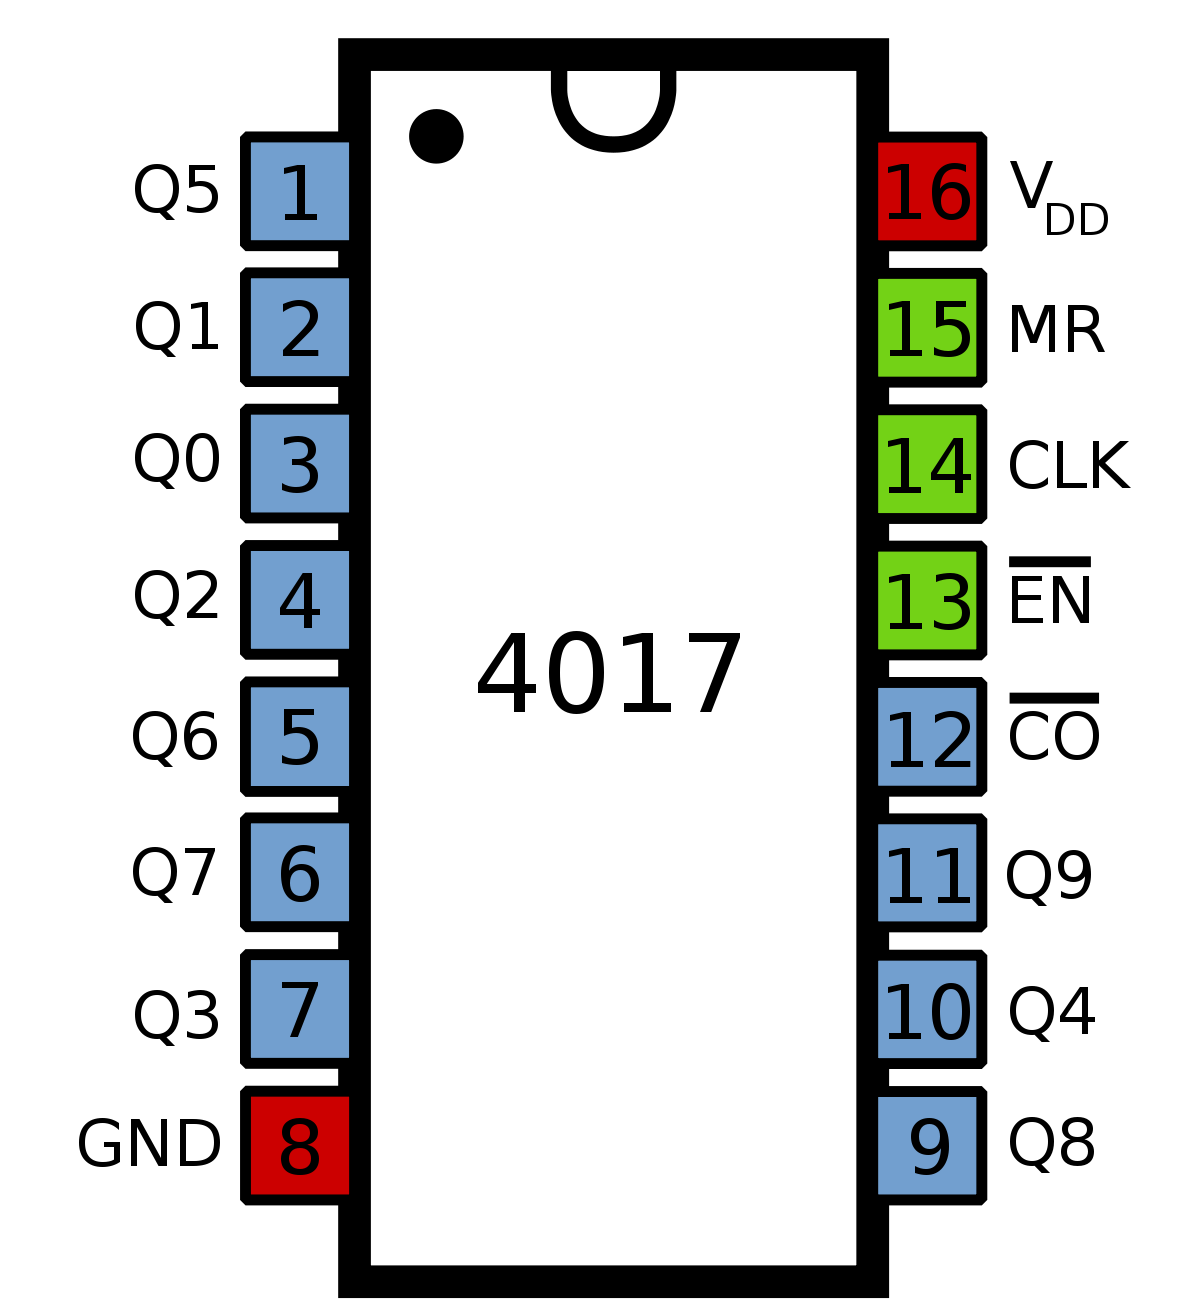
\includegraphics[width=0.5\linewidth]{4017.png}
            \caption{\label{fig:boat1}PIN chart of IC 4017}
        \end{figure}
        \begin{table}[ht]
            \centering
            \begin{tabular}{ | l | l | p{6cm} | }
                \hline
                Number & Name & Description \\ \hline
                1-7 and 9-11 & Output PINS Q0 to Q9 & 10 output, they are not in order, 
                so be careful when wiring \\ \hline
                8 & Vss or Ground & Grounding PIN \\ \hline
                12 & Carry out (CO) & The PIN to a high level after IC counting from 1-10. 
                Often used to trigger another count IC. \\ \hline
                13 & Clock Enable (EN) & PIN allowed. This positive PIN is low. When EN=0, 
                the circuit operates. \\ \hline
                14 & Clock & The counting circuit operates when there is a pulse from the 
                Clock PIN, which is positively edge-up, usually connected to another IC555 
                or quartz set to generate a pulse \\ \hline
                15 & Reset & Set output status to high \\ \hline
                16 & Vcc/Vdd & Connect to the source \\ 
                \hline 
            \end{tabular}
            \caption{\label{tab:third}Description of function of each IC 4017 PIN}
        \end{table}
        \newpage
        \par In summary we have the characteristics of the IC 4017 as follow:
        \linebreak
        \begin{itemize}
            \item 16-PIN CMOS decimal counter.
            \item Support 10 decoded outputs.
            \item Wide supply voltage range from 3V to 15V, usually +5V.
            \item Compatible with TTL (Transistor-transistor logic).
            \item Maximum frequency: 5,5MHz.
        \end{itemize}
        \par And what is application of IC 4017? That is:
        \linebreak
        \begin{itemize}
            \item This IC usually use in the counter circuit, timer circuit, LED matrix, LED chaser, 
            and almost the lost of other LED project.
            \item Use to make binary counter or binary decoder.
            \item Can be use to make splitters.
            \item Remote metering, cars, medical electronics.
        \end{itemize}
    \section{Quickview about clock pulse}
        In logic techniques, people use pulse signals (high and low) to operate. This signal is called a pulse. 
        \linebreak
        \par As you can see, the clock has an effect on the signal transmittion. Specifically, the higher 
        frequency of the clock, the faster amount of signal transmitted. 
        \linebreak
        \par For synchronous design systems, the clock is a global clock that allows all the components 
        on it to communicate and control with each other. 
        \linebreak
        \par As for the asynchronous setting system, the clock pulse is just a handshake pulse to 
        communicate between 2 components (local clock) with each other, absolutely no clock pulse for 
        the entire system. 
        \newpage
        \begin{figure}[ht]
            \centering
            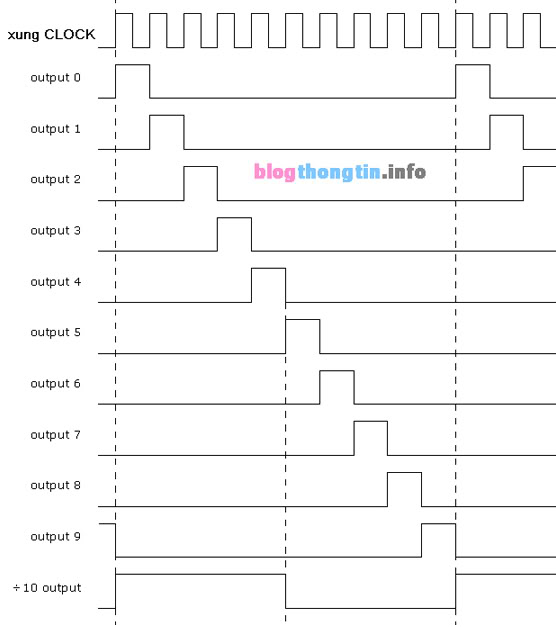
\includegraphics[width=0.5\linewidth]{n2.jpg}
            \caption{\label{fig:boat2}Output signal format according to pulse input signal of IC 4017}
        \end{figure}
        \par This is signal when IC is operated by an edge-up shock (the pulse from level 0 to level 1). 
        \linebreak
        \par PIN 13 (pin E) is the PIN that allow the IC to work, to activate this pin we have to connect 
        this pin to level 0 (also known as mass level).
        \linebreak
        \par MR pin or can be understood as Reset pin, when we give it a voltage of 1 (5V), the output Q 
        will be reset, the output Q0 is default at 1, the remaining outputs are at 0 if we do not need to use 
        the MR pin, we should connect this PIN to the mass. The diagram above we use MR pin to control 
        the 4th counting so we connect MR to Q4 pin.
        \linebreak
        \par CO pin used to connect with other IC 4017 depending on the design needs of each person, for 
        example when we need more counting of IC 4017 then we will use this pin (just connect the CO pin of this 4017 to the CLK pin of the next IC 4017).
        \linebreak
        \par As shown in the picture we see when the output pulse of the IC is simulated to a high level 
        (level 1) so continuously until the output of the IC and will return to the beginning and so on, 
        if it granted, it will be run continuously.
        \linebreak
    \section{IC NE555}
        \begin{figure}[ht]
            \centering
            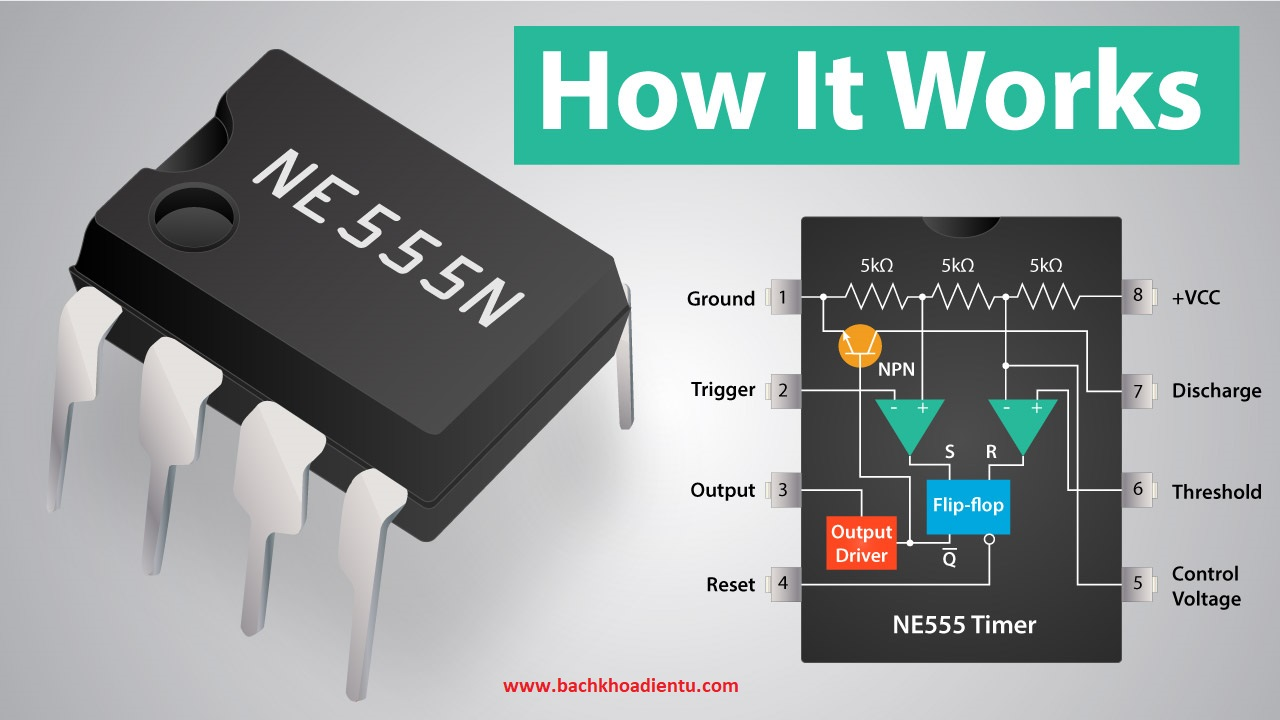
\includegraphics[width=0.5\linewidth]{555.jpg}
            \caption{\label{fig:boat3}Image and structure of IC NE555}
        \end{figure}
        \par NE555 Timer IC is an intergrated circuit (chip) used in a variety of timer, pulse generation, 
        and application oscillators. NE555 can be used to provide time lags, like an oscillators and as a 
        flip-flop element.
        \linebreak
        \par IC NE555 has been in 1972 by Signetics Corporation with 2 product lines SE555/NE555 and 
        is called time machine and is also the first available. It provides electronic circuit designers 
        with relatively cheap, stable cost.
        \linebreak
        \par Its structure is composed of OP-AMP comparing voltage, flip circuit and transistor for discharging 
        electricity like a image down here: 
        \begin{figure}[ht]
            \centering
            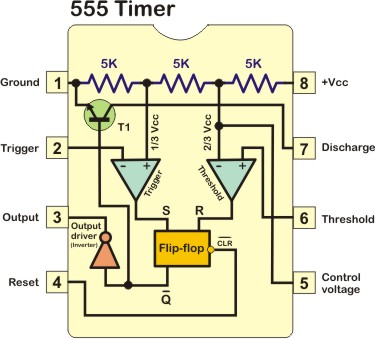
\includegraphics[width=0.6\linewidth]{inside_the_555_timer.jpg}
            \caption{\label{fig:boat4}Structure inside of NE555}
        \end{figure}
        \linebreak
        \par Depending on the manufacturer, NE555 has a different structure. Typically, the standard 
        NE555 include 25 transistors, 2 diodes, and 15 resistors on silicon processors installed in the 
        8-pin dual package (DIP-8). Variations include 556 (one DIP-14 combining tow complete 555s on one chip), 
        and 558/559 (both DIP-16 incorporating four reduced function timers on one chip).
        \linebreak 
        \par NE555 parts are temperature range from 0$^{\circ}$C to 70$^{\circ}$C and NE555 parts are 
        assigned the best temperature range from -55$^{\circ}$C to 125$^{\circ}$.
        \linebreak
        \par Low-power CMOS types of NE555 are also available, such as Intersil ICM7555 and Texas LM555, 
        TLC555, TLC551. The CMOS timer uses less power than the bipolar timer. The CMOS timer also causes 
        less noise than the dipole type when the output transitions.
        \begin{table}[ht] 
            \centering
            \begin{tabular}{ | l | l | l | p{7cm} | }
                \hline
                PIN & PIN Name & PIN direction & PIN purpose \\ \hline
                1 & GND & Ground & Supply voltage: 0V \\ \hline
                2 & TRIG & Input & Activate: when the voltage at this PIN decrease 1/2 of battery voltage CONT 
                (1/3 Vcc unless CONT have activate by outside signal). \\ \hline
                3 & OUT & Output & This is a push-pull output that is led to a low or high state (positive supply on the Vcc PIN minus about 1.7). \\ \hline
                4 & Reset & Reset & The time interval can be reset by bringing this PIN to GND, but the time does not 
                start again until this PIN rises to about 0.7V. This PIN overrides TRIG and Threshold. This PIN 
                is not used much, so it is often connected to Vcc to prevent electrical noise from causing repetition. \\ \hline
                5 & CTRL & Input & This PIN provides access to internal voltage (2/3 Vcc by default). Apply this 
                voltage to CONT, we can change the time characteristics of the device. \\ \hline
                6 & THRES & Input & Threshold: when this voltage at PIN is greater than the voltage at the CONT 
                PIN (2/3 Vcc), then the interval time ends. \\ \hline
                7 & DIS & Output & Discharge: this is the output of an open collector (OC), used to discharge 
                capacitors between intervals, in phase with the output. \\ \hline
                8 & Vcc & Source & The guaranteed voltage range of bipolar timers is usually 4.5-1.5V (some timers are specified for up to 16V or 18V), 
                although most will work as low as 3V. \\ 
                \hline
            \end{tabular}
            \caption{\label{tab:four}Describe the function of each IC NE555 pin}
        \end{table}

\end{document}